\section{Pinch Effect}
\begin{frame} {Z-Pinch}
    \begin{itemize}
        \item Current generates $B$ field in $\theta$ direction.
        \item $\mathbf{J\times B}$ points radially inward.
    \end{itemize}
    \begin{figure}
        \centering
        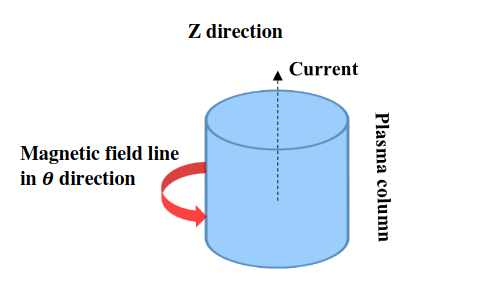
\includegraphics[width=0.7\textwidth]{figures/z-pinch.png}
        \caption{A Z-pinch in cylindrical coordinates. \cite{behbahani_2017_enhancement}}
        \label{fig:z-pinch}
    \end{figure}
\end{frame}

\begin{frame} {$\theta$-Pinch}
    \begin{itemize}
        \item Plasma current generates $B$ field in z direction.
        \item Current in primary loop together with $B$ field creates radially inward force.
    \end{itemize}
    \begin{figure}
        \centering
        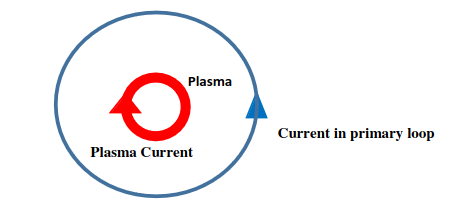
\includegraphics[width=0.7\textwidth]{figures/theta-pinch.png}
        \caption{A Schematic of theta pinch configuration. \cite{behbahani_2017_enhancement}}
        \label{fig:theta-pinch}
    \end{figure}
\end{frame}

\begin{frame} {$X$-Pinch}
    \begin{figure}
        \centering
        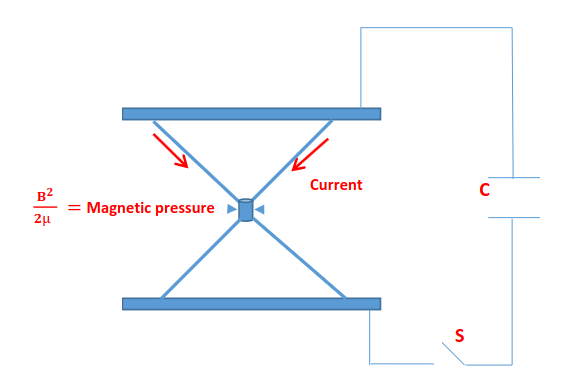
\includegraphics[width=0.7\textwidth]{figures/x-pinch.png}
        \caption{The configuration of an X-pinch device. \cite{behbahani_2017_enhancement}}
        \label{fig:x-pinch}
    \end{figure}
\end{frame}